\documentclass{article}

\usepackage[utf8]{inputenc}
\usepackage{hyperref}
\hypersetup{pdfauthor={Cristian Adrián Ontivero}}
\usepackage[yyyymmdd,hhmmss]{datetime}
\usepackage[spanish,es-tabla]{babel}
\usepackage{graphicx}
\usepackage{float}
\usepackage{color}
\usepackage{epigraph}
\graphicspath{{imgs/}}

\definecolor{darkblue}{RGB}{49,130,189}

\newlength\tindent
\setlength{\tindent}{\parindent}
\setlength{\parindent}{0pt}
\renewcommand{\indent}{\hspace*{\tindent}}

\renewcommand*{\tableautorefname}{Tabla}

%These tell TeX which packages to use.
\usepackage{array,epsfig}
\usepackage{amsmath}
\usepackage{amsfonts}
\usepackage{amssymb}
\usepackage{amsxtra}
\usepackage{amsthm}
\usepackage{mathrsfs}
\usepackage{color}

%Here I define some theorem styles and shortcut commands for symbols I use often
\theoremstyle{definition}
\newtheorem{defn}{Definición}
\newtheorem{thm}{Teorema}
\newtheorem{cor}{Corolario}
\newtheorem*{rmk}{Remark}
\newtheorem{lem}{Lema}
\newtheorem*{joke}{Joke}

\newtheorem{ex}{Ejemplo}
\newcommand{\exautorefname}{Ejemplo}

\newtheorem*{soln}{Solución}
\newtheorem{prop}{Proposición}

\newcommand{\lra}{\longrightarrow}
\newcommand{\ra}{\rightarrow}
\newcommand{\surj}{\twoheadrightarrow}
\newcommand{\graph}{\mathrm{graph}}
\newcommand{\bb}[1]{\mathbb{#1}}
\newcommand{\Z}{\bb{Z}}
\newcommand{\Q}{\bb{Q}}
\newcommand{\R}{\bb{R}}
\newcommand{\C}{\bb{C}}
\newcommand{\N}{\bb{N}}
\newcommand{\M}{\mathbf{M}}
\newcommand{\m}{\mathbf{m}}
\newcommand{\MM}{\mathscr{M}}
\newcommand{\HH}{\mathscr{H}}
\newcommand{\Om}{\Omega}
\newcommand{\Ho}{\in\HH(\Om)}
\newcommand{\bd}{\partial}
\newcommand{\del}{\partial}
\newcommand{\bardel}{\overline\partial}
\newcommand{\textdf}[1]{\textbf{\textsf{#1}}\index{#1}}
\newcommand{\img}{\mathrm{img}}
\newcommand{\ip}[2]{\left\langle{#1},{#2}\right\rangle}
\newcommand{\inter}[1]{\mathrm{int}{#1}}
\newcommand{\exter}[1]{\mathrm{ext}{#1}}
\newcommand{\cl}[1]{\mathrm{cl}{#1}}
\newcommand{\ds}{\displaystyle}
\newcommand{\vol}{\mathrm{vol}}
\newcommand{\cnt}{\mathrm{ct}}
\newcommand{\osc}{\mathrm{osc}}
\newcommand{\LL}{\mathbf{L}}
\newcommand{\UU}{\mathbf{U}}
\newcommand{\support}{\mathrm{support}}
\newcommand{\AND}{\;\wedge\;}
\newcommand{\OR}{\;\vee\;}
\newcommand{\Oset}{\varnothing}
\newcommand{\st}{\ni}
\newcommand{\wh}{\widehat}

%Pagination stuff.
\setlength{\topmargin}{-.3 in}
\setlength{\oddsidemargin}{0in}
\setlength{\evensidemargin}{0in}
\setlength{\textheight}{9.in}
\setlength{\textwidth}{6.5in}
\pagestyle{empty}



\begin{document}


\begin{center}
\Large Criptografía y Seguridad (72.44)\\[.05cm]
Apuntes sobre Seguridad en Aplicaciones\\[.05cm]
\the\year
\end{center}

\vspace{0.2 cm}
%\section{Cross-Site Scripting}
\section{Cross-Site Request Forgery}
El Cross-Site Request Forgery (CSRF\footnote{Abreviado como XSRF por algunos, se
  pronuncia ``sea-surf'' de acuerdo a quien lo acuñó. Otros nombres menos usados
  son \textit{one-click attack}, \textit{session riding}, o \textit{hostile
linking}. En español se conoce como falsificación de petición en sitios
cruzados.}) es un ataque que provoca que un navegador realice acciones sin
consentimiento del usuario sobre una aplicación en la que se encuentra
autenticado.

\begin{ex}\label{ex:1}
  En la \autoref{fig:ex} se tiene el esquema de un caso básico. Supongamos que
  hay una página llamada \verb+ejemplo.com+. Esta página
  permite a sus usuarios eliminar su cuenta, y para esto utiliza un GET a
  \verb+ejemplo.com/account/delete+. El usuario ingresa a su cuenta, y luego sin
  deslogearse de la misma, cierra la ventana y visita \verb+evil.com+, la página
  del atacante. Oculto en esta página, se encuentra el código: 

  \begin{center}
\verb+<img style="display:none" src="https://ejemplo.com/account/delete">+
  \end{center}

 Al leer  esto, el navegador realiza el GET a \verb+ejemplo.com+, la página web
 toma el request como válido (ya que el navegador envía la cookie que la página
 usa para que el usuario se autentique), y su cuenta se elimina.
\end{ex}

\begin{figure}[h]
  \caption{Ejemplo}\vspace{.2cm}\label{fig:ex}
\centering
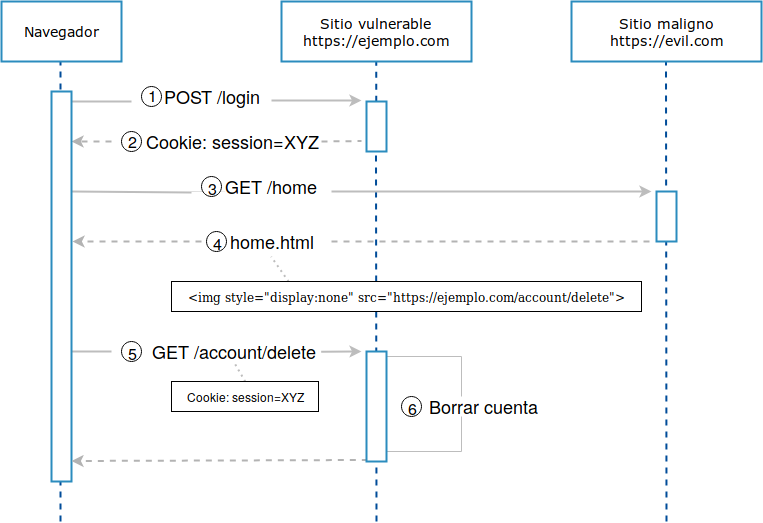
\includegraphics[width=.9\textwidth]{ex1}
\end{figure}

CSRF puede pensarse como la vulnerabilidad dual a XSS: mientras XSS abusa de la
confianza que el usuario tiene en la página o aplicación, CSRF abusa de la
confianza que la aplicación tiene en el usuario.

Las formas más comunes de explotar esta vulnerabilidad son mediante:
\begin{enumerate}
\item el atributo \verb+src+ de diferentes elementos:
\begin{itemize}
	\item \verb+<img src="http://host/?command">+
	\item \verb+<script src="http://host/?command">+
	\item \verb+<iframe src="http://host/?command">+
\end{itemize}
\item un objeto \verb+Image+:
  \begin{verbatim}
  <script>
      const img = new Image();
      img.src = "http://host/?command";
  </script>
  \end{verbatim}
\item un objeto \verb+XMLHttpRequest+:
  \begin{verbatim}
  <script>
      const postData = "name=value";
      const xhr = new XMLHttpRequest();
      xhr.open("POST", "https://example.com/shop/voteForProduct", false);
      xhr.withCredentials = true;
      const params = "productId=1337&vote=AAA";
      xhr.send(params);
  </script>
  \end{verbatim}
\item un \verb+form+ oculto que se envía automáticamente:
  \begin{verbatim}
  <form method="POST" id="ezpz" name="ezpz"
   action="https://socialnetwork.com/user/passwordchange">
      <input type="hidden" name="newpass" value="hacked">
  </form>
  <script>document.ezpz.submit()</script>
  \end{verbatim}
\end{enumerate}

Notese que en el \autoref{ex:1} se estaba utilizando un GET de manera
incorrecta de acuerdo a la especificación de HTTP. GET es uno de los
denominados \textit{safe methods} listados en \cite{rfc7231}, por lo que no
debería usarse para cambiar estado en el servidor. Esto, además de ser buena
práctica, nos lleva a una primera medida de prevención:

\begin{center}
\textbf{No usar métodos seguros como GET para modificar estado en el
servidor.}
\end{center}

Hacer esto nos asegura que el atacante no puede hacer un CSRF de forma
automática sin el uso de JavaScript.

Aun así, si bien esto es un buen primer paso preventivo, no es suficiente.

\subsection{Prevención}
Varios métodos de prevención se desarollaron a través de los años, y cuentan con
diferentes niveles de soporte en navegadores. Es importante tener presente que
ninguna de las prevenciones estandar contra CSRF sirven si existe el atacante tiene la
posibilidad de realizar un XSS, por lo que es primordial cubrirse ante estos.

\subsubsection{Recomendaciones de OWASP}
El Open Web Application Security Project \cite{owasp} recomienda dos medidas
contra los CSRF, en el orden de prioridad listados:

\begin{enumerate}
  \item Corroborar headers estandar para verificar que el request es del mismo origen.
  \item Usar algún método adicional específico contra CSRFs.
\end{enumerate}

\paragraph{Digresión sobre origenes} En \cite{rfc6454} se define que dos recursos son parte del mismo
origen si poseen el mismo protocolo, host, y puerto. En la \autoref{tab:origin} se pueden ver
algunos ejemplos de comparaciones con \texttt{http://store.company.com/dir/page.html}.

\begin{table}[H]
\centering
\caption{Comparación de origenes con
\texttt{http://store.company.com/dir/page.html}.}\label{tab:origin}\vspace{.2cm}
\begin{tabular}{lll}
URL & Resultado & Razón \\ \hline
\texttt{http://store.company.com/dir2/other.html} & Coinciden & - \\
\texttt{http://store.company.com/dir/inner/another.html} & Coinciden & - \\
\texttt{\textcolor{darkblue}{\underline{https}}://store.company.com/secure.html} & No Coinciden & Protocolos difieren \\
\texttt{http://\textcolor{darkblue}{\underline{news}}.company.com/dir/other.html} & No Coinciden & Hosts difieren \\
\texttt{http://store.company.com:\textcolor{darkblue}{\underline{81}}/dir/etc.html} & No Coinciden & Puertos difieren \\
\end{tabular}
\end{table}

Originalmente se usaba el header \texttt{Referer} para saber de dónde venía el
request. Desafortunadamente, este header se envía con todos los métodos HTTP e
incluye el \textit{path} y los \textit{query parameters} de la URL previa, lo
cual no provee seguridad extra contra ataques CSRF, y es criticado por invadir la privacidad
del usuario (el segundo sitio web puede saber sobre la actividad del usuario
en el sitio previo). Por estas razones, algunos proxies eliminan el header
(mayoritariamente cuando no se usa HTTPS), o usuarios usan extensiones que lo
suprimen del lado del cliente, por lo que no siempre se puede confiar en su
presencia.

Actualmente, los navegadores soportan el header \texttt{Origin}, que a
diferencia de \texttt{Referer}, solo se envía al hacer POST, y no incluye el
path ni los query parameters, mejorando la privacidad del usuario.

Es importante remarcar que ambos headers pertenecen al grupo de
\textit{forbidden header names} \cite{fetch}, por lo que no pueden ser modificados
programáticamente (estan bajo control exclusivo del navegador). Caso
contrario, el atacante podría simplemente modificarlos mediante un script,
tornandolos inservibles en la defensa que se describe a continuación.

\paragraph{Comparación de origenes} La primer medida robusta de
prevención es comparar el \textit{source origin} con el \textit{target origin}.
Si ambos coinciden, se acepta el request (ya que vino de dentro del
sitio mismo), de lo contrario, se lo rechaza.
El source origin se toma del header \verb+Origin+; si no esta presente, se lo
toma del header \verb+Referer+.
Dependiendo de la aplicación, el target origin puede ser una constante conocida
en tiempo de compilación, puede obtenerse de la URL del request, o puede
requerir de más trabajo si, por ejemplo, el servidor cuenta con varias
instancias o se encuentra detrás de un proxy. Para mayor detalle, referirse a
\cite{owasp}.

En los casos en que no haya ni \verb+Origin+ ni \verb+Referer+ entre los
headers, se puede tanto aceptar como rechazar la petición, pero lo seguro (y
recomendado por OWASP) es rechazarlo.

\paragraph{Defensa adicional} Esta medida se recomienda una vez implementada la
previamente descripta. Si bien el OWASP lista cuatro variantes, nos limitaremos
a describir la conocida como \textit{double cookie defense}, que posee la
ventaja de no requerir guardar estado adicional del lado del servidor. Para el
resto de las variantes, referirse al \textit{cheat sheet} de OWASP.

\paragraph{Nota sobre frameworks} Cabe mencionar que existen frameworks (e.g.
CSRF Guard para Java) que implementan las defensas previamente explicadas (o
alguna variante de las mismas), por lo que puede ser conveniente delegar la
prevención en alguno de estos. Aun así, es importante saber qué medidas de
prevención existen, con sus pros y contras, para entender si la seguridad que
otorga el framework es la necesaria, y si se lo está usando correctamente.
%\epigraph{\textit{Never inventing your own} is one of the most quoted rules of
%cryptography, but it \textit{should} be an accepted rule of development security
%in general}{Rich Lundeen}

\subsubsection{Directiva \texttt{SameSite} para cookies}
Definida en \cite{ietf}, esta directiva le indica al navegador nunca enviar una cookie cuando se realiza
un request desde una URL externa (\textit{cross-site}). Un ejemplo de uso sería:
\begin{verbatim}
  Set-Cookie: session_cookie=d34db33f; path=/; SameSite
\end{verbatim}

Esta galletita viene en dos sabores: \verb+SameSite=strict+, y
\verb+SameSite=lax+. Cuando usamos \verb+strict+, la cookie se envía solo si el request viene del
mismo sitio, mientras que con \verb+lax+ se envía también desde otros sitios,
siempre y cuando:
\begin{enumerate}
  \item El método usado sea uno de los seguros (GET, HEAD, OPTIONS, TRACE).
  \item La petición HTTP sea a un \textit{top-level browsing context}.
\end{enumerate}
Ante la falta de atributo, o un atributo inválido, el valor predeterminado es
\verb+strict+.

\paragraph{SameSite contra CSRF} Una forma de utilizar \verb+SameSite+ para
evitar ataques CSRF es tener dos cookies en lugar de una. La primera puede no
usar \verb+SameSite+, o hacerlo con el atributo \verb+lax+, y ser usada para
permitir al usuario navegar. La segunda se marcaría con \verb+SameSite+ (en
\verb+strict+), y su ausencia requeriría al usuario reautenticarse previo a
acciones con efectos secundarios (o no idempotentes). Conceptualmente, la
primera otorga permisos de lectura, mientras que la segunda, permisos de
escritura.

Si bien aun no cuenta con soporte de la mayoría de los navegadores, puede
aprovecharse para aquellos que si, y a medida que los navegadores lo
implementen, se espera que sea una media efectiva de prevención.

\subsubsection{Defensas con interacción del usuario}
Las medidas de prevención antes mencionadas son imperceptibles para el usuario,
por lo que son preferibles desde un punto de vista de usabilidad. Existen otras,
que a pesar de resultar más engorrosas para el usuario, tienen sus usos. Un
ejemplo típico es requerir la contraseña actual antes de poder cambiarla. Otra
posibilidad es pedir al usuario completar un CAPTCHA.\ En general, cualquier
medida del estilo ``desafío-respuesta'' (\textit{challenge-response}), que no
pueda ser predecido por el atacante, es efectivo. No obstante, su uso suele
restringirse a operaciones de alto riesgo (e.g.\ transferencias bancarias) por afectar la
experiencia del usuario.

\subsection{Notas Finales}

El header HTTP \texttt{Origin} fue propuesto en \cite{Barth}, y posteriormente
definido en \cite{rfc6454}. En \cite{Barth} también se describe un ataque
llamado \textit{login CSRF}, en el que el atacante hace que la victima ingrese
con la cuenta del atacante (referirse al paper para mayor detalle).
Cuatro casos de vulnerabilidades pueden leerse en \cite{Zeller}.
Otros documentos como \cite{Burns,Blatz} también son instructivos, pero algunas
recomendaciones estan desactualizadas, por lo que a la hora de implementar una
defensa, se recomienda referirse al OWASP.\
A pesar de ser robusta, por sí sola la defensa de doble cookie presentada es
vulnerable a \textit{man-in-the-middle attacks} por HTTP, y XSS en subdominios.
Para más detalles referirse a \cite{Johansson}.

\paragraph{Origen} Norm Hardy publicó en 1988 un documento sobre un problem de
permisos al nivel de aplicación que denominó diputado confundido
(\textit{confused deputy}) \cite{Hardy}. Luego, durante el 2000 en un correo en
bugtraq \cite{bugtraq} se describió cómo ZOPE, al igual que otras páginas, se
veían afectadas por un problema del estilo diputado confundido, que hoy se
conoce como una vulnerabilidad CSRF.\ El término \textit{Cross-site Request Forgery} fue acuñado por Peter Watkins un año más tarde nuevamente en bugtraq
\cite{watkins}, como respuesta a un correo cuyo asunto era \textit{The Dangers of Allowing Users to Post Images}.
\bibliography{refs}
\bibliographystyle{unsrt}

\end{document}


